\chapter{Proiectare de detaliu și implementare}
\pagestyle{fancy}

Acest capitol prezinta in detaliu solutia propusa pentru un sistem de monitorizare a temperaturii si a umiditatii. Aceasta include protocoalele de 
comunicatie utilizate, limbajele de programare si arhitecturi de abstractizare.

Arhitectura generala a sistemului este compusa din 5 componente pricipale descrise succint in cele ce urmeaza:
\begin{itemize}
	\item Aplicatie Android - reprezinta interfata cu utilizatorul.
	\item MQTT Broker - reprezinta un server specializat pe protocolul de comunicatie MQTT.
	\item Server - reprezinta un server pentru comunicatia cu baza de date
	\item Baza de date - reprezinta locul si modul in care sunt stocate datele.
	\item Senzor - reprezinta un dispozitiv care are capabilitatea de a achizitiona temperatura si umiditatea dintr-un mediu si de a comunica cu un router.
\end{itemize}

Figura \ref{fig:ArhitecturaGenerala} prezinta arhitectura generala a sistemului 
\begin{figure}[H]
    \centering
    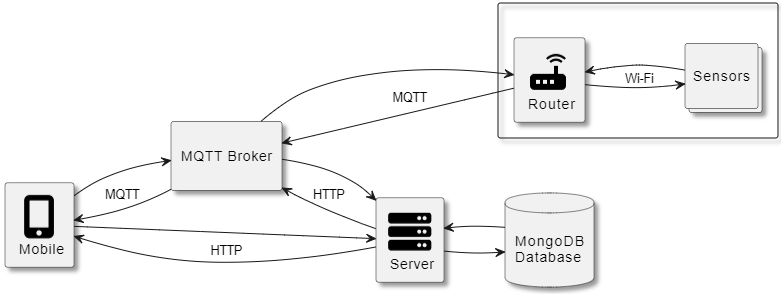
\includegraphics[scale=0.76]{figs/ArhitecturaGenerala.png}
    \caption{Arhitectura generala a proiectului}
    \label{fig:ArhitecturaGenerala}
\end{figure}


{\color{blue}Împreună cu capitolul \textbf{precedent} și cel \textbf{următor} trebuie să reprezinte aproximativ 70\% din total.\\}

Scopul acestui capitol este de a documenta aplicația dezvoltată în așa fel încât dezvoltarea și întreținerea ulterioară să fie posibile.
Cititorul trebuie să identifice funcțiile principale ale aplicației din ceea ce este scris aici.
Capitolul ar trebui sa conțină (nu se rezumă neapărat la):
\begin{itemize}
	\item schema generală a aplicației
	\item descrierea fiecărei componente implementate, la nivel de modul
	\item diagrame de clase, clase importante și metode ale claselor importante.
    \item diagrame de baze de date
\end{itemize}
